\algorithm{The Robust Object Watermarking Algorithm}%
          {Balamurugan Chirtsabesan, Tapas Sahoo}


\section{Introduction}
The Robust Object Watermarking presents a new approach to watermarking.
Instead of applying the watermarking scheme to the raw code directly, a new
vector representation of the code is created. The basic idea revolving
around this scheme is that instead of considering the overall structure of
the code and its control flow, the code is viewed as a statistical object.
The frequencies of groups of instructions in the entire code are taken into
consideration in creating a new vector representation of the data. Spreading
the watermark throughout the target code ensures a large measure of security
against intentional and unintentional attacks.

\begin{description}
   \item[Identifying the Vector instruction Groups: ]
      A set of instruction groups are identified that will form the 
      watermark vector to be embedded. Ideally these instructions groups are instructions 
      which have frequent occurence in the code and are chosen from some 
      profiling information of the code. These instruction groups are 
      small, each containing number of instructions in the range 1 to 4. This
      maximizes the probability of occurence of the instruction groups in the 
      code while preserving the stealth.
   \item[Building the CodeBook: ] 
      The CodeBook contains a mapping between semantically equivalent sets of
      instructions and is constructed in accordance with the vector instruction
      groups mentioned above. The basic motivation behind the construction of
      such a CodeBook is to facilitate the insertion of the watermark vector 
      instructions through code subsitution.  The CodeBook has been designed
      such that it can be upgraded as and when the vector instruction group is
      upgraded and new possible code equivalence is identified.
   \item[Vector Extraction: ] In this step, the vector length is chosen, the 
      length of which is constrained by the number of the vector instruction 
      groups. The frequency of occurence of the vector instruction groups  in 
      the code are identified and the intial vector is formed out of it. 
   \item[Insertion: ] In this step, the watermark vector selected is to be 
      embedded in the code. The frequencies of instructions in the vector 
      instruction group are varied in accordance with the watermark vector by
      different implementation techniques such as code subsitution, new code
      insertion, cloning of method, etc. Care must be taken to ensure that all
      the operations done do not violate the semantics of the code.
   \item[Recognition:] 
      During recognition, the Vector Extraction procedure is invoked to 
      extract the frequencies of the instructions in the vector group. The 
      watermark is identified across a certain level of tolerance. A threshold
      is set prior to the extraction. Ideally, the watermark should be passed
      and the recognizer verifies the code and answers if the watermark vector 
      is still present in the code within the threshold boundary.
\end{description}


\begin{figure}
\begin{listing}{1}
package sandmark.watermark.objectwm;

public class ObjectWatermark extends sandmark.watermark.StaticWatermarker {

   public ObjectWatermark();

   public String getShortName();
   public String getLongName();

   public static sandmark.util.ConfigProperties getProperties();
   public static void setProperties(sandmark.util.ConfigProperties);

   public sandmark.util.ConfigProperties getConfigProperties();
   public void setConfigProperties(sandmark.util.ConfigProperties);

   public java.lang.String getAlgHTML();

   public java.lang.String getAlgURL();

   public void embed(java.util.Properties);
      - Procedure to embed the watermark. Invokes the APIs in the Insertion class.

   public java.util.Iterator recognize(java.util.Properties);
      - Procedure for watermark recognizing.

   class Recognizer implements java.util.Iterator {
      public Recognizer(String jarInput);
      public void generate();
      public boolean hasNext();
      public java.lang.Object next();
   }
}
\end{listing}
\caption{The general APIs used for implementing Algorithm for Robust Object Watermarking.}
label{}
\end{figure}


\section{Vector Instruction Group Identification }
The instruction groups are identified keeping in mind the probability
of occurence of the instructions in the code which is to be watermarked. Each 
vector group contains atmost 4 instructions. This is because a greater number of
instructions in a vector group has less likelihood of occurence in the code. We
have at present identified 8 vector instruction groups. The implementation has 
been done such that new groups can be appended to the existing vector groups as
and when identified. The number of vector groups denotes the length of the
watermark vector  than can be embedded in the code.

\section{Building the CodeBook : } The CodeBook construction goes in parallel
with the identification of the Vector Instruction Groups. Set of instructions 
are identified which are semantically equivalent and are placed in the same set.
Moreover the equivalence should be such that it facilitates the increase of 
instruction vector frequencies. The following points are taken into 
consideration while building the CodeBook.

\begin{itemize}
   \item [1.] Each vector instruction group is dependent on atleast one CodeBook
              instruction group for its insertion. 
   \item [2.] Each instruction set in the CodeBook services exactly one vector
              instruction group. This simplifies the insertion procedure and
	      isolates the frequency updates of different vector groups.
   \item [3.] Each group in the CodeBook contains a set of instruction which 
              has high frequency of occurence in the code. This gives more 
	      oppurtunities for code subsitution rather than new code insertion
	      for vector frequency increment.
   \item [4.] The code substitution increases the size of the code,but minimally.
   \item [5.] The CodeBook has been designed such that it can be upgraded as 
              and when new groups are identified with minimal effect on the 
	      APIs accessing the CodeBook.
\end{itemize}

\begin{figure}
\begin{listing}{1}
package sandmark.watermark.objectwm;

public class CodeBook {

   CodeBook();
      - defines the CodeBook ie. the CodeGroup instruction groups, the vector 
        group instruction groups and the dependencies between them.

   int getInstructionFromCodeBook(String[], int, int, int);
      - invoked from the Insertion class to access the CodeBook.

      private String[][] getParams(String[], int);

      private String[] putParams(String[], int, String[][]);

}
\end{listing}
\caption{The above figure shows the different APIs used for CodeBook access.}
\label{}
\end{figure}


A dependency array stores the dependence between each Vector Group Instruction
and the set of CodeBook Instructions.

\section{Vector Extraction }
The vector extraction procedure is invoked at the initial stage prior to watermark
insertion and during watermark recognition. The entire code is scanned for the 
occurence of the Vector Instruction Groups and the vector components are formed out
of the frequencies of the corresponding groups.
\begin{figure}
\begin{listing}{1}
package sandmark.watermark.objectwm;

public class vectorExtraction {

   public static java.util.Vector extractVector(String);
      - implements the vector extraction procedure
}
\end{listing}
\caption{VectorExtraction APIs}
\label{}
\end{figure}

\section{The overall watermarking algorithm }
{\em Vector Extraction: } Define $n$ as a security parameter. Define a set $S$ of
$n$ ordered groups of machine language instructions. For each group $i$ in $S$,
compute the frequency $c_i$ of the group in the code, and form the vector $c = 
(c_1, \ldots, c_n)$. This $c$ is the extracted vector. 
\\\\
{\bf {\em Algorithm}}
\\
{\em Initialization:} Set a detection threshold $\sigma $.
\\
{\em Watermark Insertion:}
\begin{itemize}
\item
Apply the vector extraction step to obtain a vector $c$ (of length $n$).
\item
Choose an $n$ coordinates vector $w = (w_1, \ldots , w_n)$ whose coefficients
are randomly distributed following a normal law with standard deviation $\alpha$.
\item
Modify the code in such a way that the new extracted vector $\overline c$ is $c + w$.
\end{itemize}
{\em Watermark Testing:}
\begin{itemize}
\item
Apply the extraction step to obtain a vector $d$.
\item
Compute a simliarity measure $Q$ between $d -\overline c$ and $w$.
\item
If $Q$ is higher than $\sigma$ then the algorithm outputs $marked$, else it
outputs $unmarked$.
\end{itemize}


\section{Insertion } The insertion procedure is the most crucial step in
the entire watermarking algorithm. For each Vector Instruction Group of the
watermark vector, the algorithm intends to increase the frequency of that group
by the vector value. It resorts to three techiniques to increase the vector 
group frequency.
\begin{itemize}
   \item {\bf {\em Code substitution: }}  In this techinique we looks for group of 
         instructions in the code that can be substituted by a equivalent set of
	 instructions as enumerated in the CodeBook to increase the vector 
	 frequency. As an example, say vector group $A$ is dependent on the 
	 CodeGroup[i,j]. We look for the occurence of CodeGroup[i,0] and 
	 substitute it by the equivalent set of instructions in the 
	 CodeGroup[i,j]. This increases the frequency of the vector by one. Some
	 issues which we deal with while doing the substitution are enumerated 
	 below:
	 \begin{itemize}
	 \item [1.] We handle jump to a target out from this set of instructions
	       appropriately by saving target instruction handles and later
	       replacing it in the substituting instruction set. 
         \item [2.] At present we do not handle jumps into the instruction set.
	       So we discard the occurence of instruction sets which have 
	       branch targets as candidates for substitutions.
         \item [3.] The substitution increases the code length minimally as per
	       the design of the CodeBook. We observed that finding an 
	       equivalence in which the vector frequency is increased as well 
	       the code size is reduced very difficult( unless the vector 
	       instruction group is restricted to almost one ).
	 \end{itemize}

         \begin{figure}
         \begin{center}
         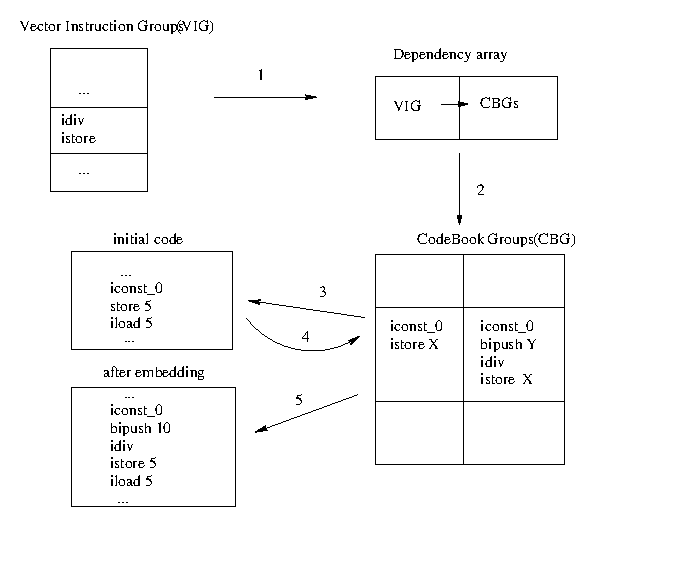
\includegraphics{fig1.eps}
         \end{center}
	 \caption{}
	 \label{}
         \end{figure}

         Depending on the CodeBook implementation and the actual occurences of
	 the instruction groups in the code there is an extent to which
	 subsitution can be done to increment the vector frequency. Once this
	 is exhausted, we resort to the next two techinques for vector increment.

   \item {\bf {\em New code insertion: }} This is the most difficult part which we 
         encountered in the entire implementation. First of all, instructions cannot be
	 inserted at any random point in the code. After embedding, the modified
	 code should pass the verifier. The following things were handled during
	 the insertion:
	 \begin{itemize}
	 \item [1.] The substituting instructions corresponding to the vector are
	       taken from the CodeBook group it is dependent on. To ensure that
	       these set of instructions do not affect the stack size, we 
	       appended the instructions with required number of $pop$ 
	       instructions.
         \item [2.] The insertion point is verified so that it does not breakup any 
	       other exisiting vector instruction group in the code.
	 \item [3.] The variables used in the instructions to be inserted need
	       to be declared and initialized in the method in which they are
	       inserted prior to their use.
         \item [4.] To preserve the semantics of the code we inserted opaque
	       predicates to jump over the newly inserted instructions. All the
	       declarations for the predicate variables are done in the start
	       of the method, though in the ideal case it could be anywhere before 
	       the point where they are used. Ideally we can have a set of such
	       predicates in pool from which we can pick one in random and 
	       plugin into the method after inserting the vector instruction
	       group codes.
	 \end{itemize}
   \item {\bf {\em Method Cloning: }}In this techinique we identify the existing methods 
         where we have occurence of the particular vector group instructions and
	 create a clone of that method. This effectively increments the vector 
	 frequency. Some issues handled during this cloning are:
	 \begin{itemize}
         \item [1.] Unlike other techniques, we have to keep track of the frequency
	       updates of all the vectors since the replication might increase the
	       vector frequencies of other vector groups.
	 \item [2.] We maintain a threshold beyond which if the frequencies are
	       modified, then we back track and do not replicate the method.
         \item [3.] Ideally, we would make a bogus call to this clone method. But we
	       do not implement such calls. In such a case a problem arises due to 
	       parameter passing. We need to initialize all the parameters in the 
	       clone method prior to all their use.
	 \end{itemize}

\end{itemize} 


\begin{figure}
\begin{listing}{1}
package sandmark.watermark.objectwm;

public class Insertion {

   public void modifyCode(java.util.Vector );
      - Entry procedure for this 'Insertion' class


   org.apache.bcel.generic.InstructionHandle getCodeSubstPoint(String[], int, String[]);
      - Searches and marks the instruction group occurence point in the code and returns the 
        instructions to be substituted. 

   void substituteCode(org.apache.bcel.generic.InstructionHandle, String[], int);
      - Subsitutes the new instructions  obtained from the codeBook into the code at the 
        marked instruction handle point.

   void newsubstituteInstruction_Embed(String[], int);
      - Implements the insertiong of previously non-existing code to increase the 
        vector frequency. This sets a random class-method-instruction insertion point for
	insertion.


      void substituteNewCode( org.apache.bcel.generic.InstructionHandle, String[], int);
         - Invoked by newsubstituteInstruction_Embed(); performs the actual low level insertion
	   operation.

         String transformCode(String);
            - invoked by substituteNewCode();  it populates the new instruction set to be 
	      embedded with valid data and returns the final instruction to be inserted.

            int getLocalVarIndex_CreateIndex();
	       - invoked by transformCode(); returns a vaild local variable index. if none 
	         exist then it creates a new one and returns its index.

        
         org.apache.bcel.generic.Instruction extractInstrType(String);
	    - This API forms the instruction object to be inserted after parsing the input
	      instruction stream and returns the object.

\end{listing}
\caption{The following APIs are implemented for the watermark Insertion procedure}
\label{}
\end{figure}

\begin{figure}
\begin{listing}{39}
         void insertOpaque( org.apache.bcel.generic.InstructionList, 
	                    org.apache.bcel.generic.InstructionHandle,
			    org.apache.bcel.generic.InstructionHandle,
			    org.apache.bcel.generic.InstructionHandle, int);
            - Generates the opaque predicate and inserts it in appropriate position.

        
	 int getOpaqueDeclPoint(int);
	    - checks for and returns a $safe$ point for new instruction insertion.
        
      boolean checkSplitVectorGrp(int, org.apache.bcel.generic.InstructionHandle[]);
         - Ensures that the insertion point for the new vector group does not split
           another existing vector instruction group in the code and consequently 
           reduce its vector freqeuency.

         
   int newcopyMethod_Embed(String[], int, int, int);
      - Implements the method cloning procedure.

   
   int remVecfreqUpdatesInThreshold(int, int);
      - Ensures that the method cloning does not update the vecotr frequencies beyond
        the {\em threshold}.

 
   /* the various support APIs for the above APIs */

   int getRandomValue(int, int);

   void getInsertLocation(Integer[]);

   int varTypeIsInt(int);

}

\end{listing}
\caption{The following APIs are implemented for the watermark Insertion procedure}
\label{}
\end{figure}

\section{Comparison with the previous implementation on x86 assembly code}
A previous implementation of this object watermarking was done in x86 assembly 
code. Each of these languages had its own constraints that restricted the 
implementation of the watermark embedding. In x86 assembly code we need to be 
careful in register selections during new instruction embedding as well
as code substitution so that they dont interfere with each other. In the
implementation we did on java bytecodes, we figured out that one needs to 
take into consideration the stack size while embedding new code. But no such 
problems arised during code substitutions which are semantically equivalent. 
The x86 code provides additional flexibility of swapping instruction sets or 
reordering instructions within an instruction group  as long as the dependencies
between the instructions are not violated, while such transformations have 
limited scope in the case of java bytecodes primarily due to the constraints of
maintaining the proper stack height.

\section{Analysis of attacks }
 The watermark faces the most serious threat from 
decompiling and recompiling the code. The compiler optimizations  may change the
 sequence of instructions and even some instructions itself. The instructions in
the vector group might well be the target of such modifications which results
 in the modification of the embedded frequency vector. But at the same time, since
 the watermark is spread across the entire code, the attacker has least idea about
the exact location of the watermark. So to effect any substantial chenge in the 
vector frequency he needs to decompile and recompile the entire code rather than
parts of the code which is tedious. Code compression poses the least threat since
code has to be decompressed again to render it executable, so the watermark 
remains intact.  

\section{Brief analysis of our work and scope for future Work } 
We followed an extremely conservative approach during watermark embedding. One
approach would have been to make an arbitrary change in the code and verify 
whether the new vector is closer to the target vector. If it digresses in the 
wrong direction then backtrack and try out another random modification. In our
approach we always made sure prior to making any modification to the code that the
resulting vector is always closer to the target vector. Such an approach was
simple as well as preserved correctness of the code in all instances. The 
ratio of the code size before and after embedding increases minimally if the 
bulk of the code modification is done through substitution rather than new
code insertion which apparently increases the code size drastically by a large
factor.  So its extremely important to identify the correct CodeBook and the 
Vector Instrution groups.  The strengh of the watermark lies in the secret 
CodeBook which is maintained since there are always a wide range of possibilities
of code equivalence and also the distribution of watermark over the entire
code rather than being concentrated at a single point in the code. This increases 
the stealth of the watermark. Also we observed that codes with lower level of
tolerance seem to withstand the tampering of this type of watermark more than code
 which provides more scope for modifications.\\\\
As a future work,  we would like to identify some sort of profiling techniques to 
identify a proper set of vector and CodeBook instructions. We would also like to
identify a few more approaches to embed the vector. The overall implementation 
needs to be modified to some extent so that we can have a  framework in which we
 can plugin new code modification techniques.

\section{Conclusion: } 
The vector extraction paradigm produces a robust watermarking technique. It mainly
takes advantage of the distribution of watermark over the code to maintain its 
stealth. But at the same time the effectiveness in the java bytecodes lies 
entirely on the exact implementation technique. 

\section{Bibliography}
\begin{itemize}
\item [1.]
Julien P. Stern, Gael Hachez, Francois Koeune, and Jean-Jacques\\ Quisquate
r. Robust Object Watermarking: Application to Code. In A. Pfitzmann, editor
, Information Hiding '99, volume 1768 of Lectures Notes in Computer Science
 (LNCS), pages 368--378, Dresden, Germany, 2000. Springer-Verlag. http://ci
teseer.nj.nec.com/stern00robust.html
\item [2.]
I. Cox, J. Kilian, T. Leighton and T. Shamoon, "A secure, robust watermark
for multimedia", in Proc. Workshop on Information Hiding, Univ. of Cambridg
e, U.K., May 30 - June 1, 1996, pp. 175-190 \\ http://citeseer.nj.nec.com/a
rticle/cox96secure.html
\end{itemize}

